% TeX root=../main.tex

\section{Sistema verbal}

\subsection{Flexão}

Até onde temos atestação no \emph{corpus}, as formas finitas do verbo luvita
flexionam em:
\begin{inparaenum}[(a)]
	\item voz: ativa e médio-passiva;
	\item tempo: presente e pretérito;
	\item modo: indicativo e imperativo.
\end{inparaenum}
Além das formas finitas, também temos em luvita o infinitivo, o gerundivo, uma
forma de substantivo verbal e particípios na voz ativa e passiva.

\paragraph{Desinências do indicativo}
A tabela a seguir contém as desinências do indicativo.\footnote{Nas tabelas a
	seguir, as formas em colchetes são particularmente raras. As formas com {?} não
	são atestadas.}
As formas médias terminadas em \emph{-si} talvez representem a adição de um
pronome reflexivo \emph{-si}, não atestada em nenhum outro contexto.

\begin{center}
	\begin{tabular}[c]{lll|ll}
		\toprule
		     & \multicolumn{2}{c|}{Presente do indicativo}           & \multicolumn{2}{c}{Pretérito do indicativo}                                                \\
		     & ativo                                                 & médio-passivo                               & ativo            & médio-passivo             \\
		\midrule
		1sg. & \emph{-wi}                                            & {?}                                         & \emph{-ha}       & \emph{-hasi}              \\
		2sg. & \emph{-si} [\emph{-tis}]                              & \emph{-ta}                                  & {?}              &                           \\
		3sg. & \emph{-di}\slash{}\emph{-ri}, [\emph{-i}, \emph{-ia}] & \emph{-ati}\slash{}\emph{-ari}              & \emph{-da, -ta}  & \emph{-asi}, \emph{-tasi} \\
		1pl. & {?}                                                   & {?}                                         & \emph{-han}{(?)} & {?}                       \\
		2pl. & \emph{-tani}                                          & {?}                                         & {?}              & {?}                       \\
		3pl. & \emph{-nti}                                           & {?}                                         & \emph{-nta}      & \emph{-antasi}            \\
		\bottomrule
	\end{tabular}
\end{center}

\noindent As formas de 3sg.pres.atv. \emph{-ri} e 2pl.pres.atv. \emph{-rani} são
rotacizadas. A forma 1pl.pres.atv. \emph{-han} talvez seja uma forma singular,
conforme proposto por~\citet{Carruba1984} \emph{contra}~\citet{MorpurgoDavies1980}.
Autores mais antigos interpretaram incorretamente a desinência
gerundiva \emph{-min{(a)}} como 1pl.pres.atv.

\paragraph{Desinências do imperativo}
A tabela a seguir contém as desinências do imperativo.

\begin{center}
	\begin{tabular}[c]{lll}
		\toprule
		     & \multicolumn{2}{c}{Imperativo}               \\
		     & ativo                          & mp.         \\
		\midrule
		2sg. & \emph{∅}                       & {?}         \\
		3sg. & \emph{-du}                     & \emph{-aru} \\
		\midrule
		2pl. & \emph{-ranu}                   & {?}         \\
		3pl. & \emph{-ntu}                    & {?}         \\
		\bottomrule
	\end{tabular}
\end{center}

\noindent A forma 2pl.imp. \emph{-ranu} é rotacizada de uma forma não atestada
*\emph{-tanu}.

\paragraph{Formas não-finitas}
As formas não finitas atestada são:

\begin{compactitem}
	\item Particípio passivo: \emph{-ama\slash{}i-}\footnote{Talvez haja uma única
		atestação de um particípio passivo em \emph{-ant-}: \emph{harwatanza}
		`viajando' (JISR EL HADID 4, §4).}
	\item Substantivo verbal: \emph{-ur-}
	\item Infinitivo: \emph{-una}
	\item Gerundivo: \emph{-min{(a)}}
\end{compactitem}



\subsection{Quadro de conjugação}

O quadro a seguir contem a conjugação do verbo \emph{izi{(ya)}-} `fazer', com as
formas do verbo \emph{la-} `pegar', \emph{tuwa-} `colocar', \emph{pi-} `dar',
\emph{as-} `ser', \emph{hwihwisa-}
`correr' e \emph{tumanti-} `escutar' onde necessário por falta de atestação.

\begin{center}
	\begin{tabular}[c]{lll|ll}
		\toprule
		     & \multicolumn{2}{c|}{Pres.\ ind.} & \multicolumn{2}{c}{Pret.\ ind.}                                              \\

		     & atv.\emph{}                      & mp\emph{}
		     & atv.\emph{}                      & mp\emph{}                                                                    \\
		\midrule
		1sg. & \emph{iziyawi}                   & {?}\emph{}                      & \emph{iziyaha}       & \emph{izihasi}      \\
		2sg. & \emph{lasi}                      & \emph{piyata}                   & {?}\emph{}           & {?}                 \\
		3sg. & \emph{izidi, piyai}              & \emph{iziyari}                  & \emph{izida, tuwata} & \emph{hwihwisatasi} \\
		1pl. & {?}                              & {?}                             & \emph{izihan}{(?)}   & {?}                 \\
		2pl. & \emph{asatani}                   & {?}                             & {?}                  & {?}                 \\
		3pl. & \emph{iziyanta}                  & {?}                             & \emph{piyanta}       & \emph{iziyantasi}   \\
		\bottomrule
	\end{tabular}
\end{center}


\begin{center}
	\begin{tabular}[c]{lll}
		\toprule
		                                        & \multicolumn{2}{c}{Imp.}                  \\
		\midrule
		2sg.                                    & \emph{iziya}             & {?}            \\
		3sg.                                    & \emph{iziyadu}           & \emph{iziyaru} \\
		2pl.                                    & \emph{tumantiranu}       & {?}            \\
		3pl.                                    & \emph{iziyantu}          & {?}            \\
		\midrule
		\midrule
		\multicolumn{2}{l}{Particípio  passivo} & {\emph{tumantimi-}}                       \\
		\multicolumn{2}{l}{Infinitivo}          & {\emph{lana}}                             \\
		\multicolumn{2}{l}{Gerundivo}           & {\emph{iziyamin{(a)}}}                    \\
		\bottomrule
	\end{tabular}
\end{center}

\subsection{Morfologia derivacional}

\paragraph{Sufixos}
Algumas formas verbais são produzidas por derivação, utilizando os seguintes
sufixos:
\begin{compactenum}[(a)]
	\item \emph{-sa-}: sentido iterativo:
	\begin{center}
		\emph{maranuha} `eu destrui' (KARKAMIŠ A1a, §9)\\
		$\downarrow$\\
		\emph{maranu\textbf{sa}ha} `eu destruí várias vezes' (TELL AHMAR 6, §6)
	\end{center}
	\item \emph{-za-}: sentido iterativo:
	\begin{center}
		\emph{waliyanta} `eles ergueram' (KARKAMIŠ A14a, §§6, \textsc{⌈}7\textsc{⌉})\\
		$\downarrow$\\
		\emph{waliya\textbf{za}nta} `eles ergueram (repetidamente)' (IZGIN 1, §18)
	\end{center}
	\item \emph{-nu{(wa)}-}: sentido causativo:
	\begin{center}
		\emph{taha} `eu ergui' (ARSUZ 1+2, §§9)\\
		$\downarrow$\\
		\emph{ta\textbf{nu}ha} `eu fiz erguer' (KARKAMIŠ A6, §19)
	\end{center}
\end{compactenum}

\paragraph{Redobro}
O redobro é utilizado por vezes para produzir o sentido iterativo:
\begin{center}
	\emph{sarlati} `ele oferece' (ANCOZ 9, §2)\\
	$\downarrow$\\
	\emph{\textbf{sa}sarlai} `ele sempre oferece' (BULGARMADEN, §11)
\end{center}

\paragraph{Prevérbios}
Prevérbios são preposições que alteram o sentido do verbo.
As mais comuns são:

\begin{multicols}{2}
	\begin{compactenum}[(a)]
		\item *\emph{anan} `abaixo, para baixo'
		\item \emph{anta} `em, dentro'
		\item \emph{antan} `para dentro'
		\item \emph{apan{(i)}} `atrás (de)'
		\item \emph{arha} `completamente, embora'
		\item CUM\emph{-ni/-i} `?'
		\item *\emph{kata} `para baixo'
		\item \emph{paran{(i)}} `na frente de'
		\item \emph{pari} `por cima'
		\item \emph{sara} `para cima'
	\end{compactenum}
\end{multicols}

\subsection{Usos}

\paragraph{Voz}
A voz ativa é utilizada para ações que o sujeito realiza.
A voz médio-passiva é usada para:
\begin{inparaenum}[(a)]
	\item ações que o sujeito realiza em proveito próprio (média);
	\item ações que o sujeito sofre (passiva).
\end{inparaenum}
A voz passiva costuma ser expressa pelo particípio passiva.


\paragraph{Tempos}
O presente expressa o presente, futuro e presente histórico (quando coordenado
com um pretérito).
O pretérito é utilizado para expressar todos os sentidos de passado bem como
estados presentes resultantes de ações pretéritas.


\paragraph{Modos}
O indicativo expressa tanto estados de coisas factuais (`fazer') quanto estados de coisas
deônticos (`dever fazer').
Ordens são expressas pelo imperativo, que também pode expressar desejos (`querer
que faça'), sobretudo na terceira pessoa.
A proibição é expressa pela sequência de \emph{nis} (NEG\textsubscript{2}) +
indicativo presente, salvo nas cartas de Assur.

\paragraph{Substantivo verbal}
A expressão de um substantivo verbal + \emph{as} `ser\slash{}estar' tem valor
deôntico: \emph{hatura asatani} `vós deveis escrever'.

\paragraph{Gerundivo}
O gerundivo sempre expressa uma obrigação e é utilizado junto do verbo \emph{as-} `ser\slash{}estar'.


\section{Partículas e clíticos}

Como é comum nas línguas anatólicas, a segunda posição de uma sentença (e por
vezes oração) é reservada para partículas e demais formas enclíticas  (i.e.\ sem
acento próprio) dispostas em uma ordem regular, ocupando a \emph{posição de Wackernagel}, também conhecida de
outras línguas indo-europeias.\footnote{O fenômeno também é conhecido como
	\emph{primeira lei de Wackernagel}. Para mais detalhes sobre a cadeia de
	clíticos em anatólico, ver~\GrHL{§30.15-21}, bem
	como~\citet{Garret1989,Garret1990,AgbayaniGolston2012}.
	Para detalhes sobre a cadeia de clíticos em outras línguas indo-europeias,
	ver a seção final de~\citet{WackernagelsLawI}.
}

A primeira posição da sentença é ocupada por um termo \emph{ortotônico},
seja um substantivo, adjetivo, pronome, verbo ou advérbio ou pelo conectivo
ortotônico \emph{a} `e'.
As posições seguintes são opcionais:
\begin{inparaenum}
	\item[2.] conectivos \emph{=ha} `e' e \emph{=pa} `mas';
	\item[3.] partícula citativa\slash{}\emph{quotative} \emph{=wa};
	\item[4.] pronomes enclíticos (os dativos precedem nominativos ou acusativos
	se houverem)
	\item[5.] a partícula locativa \emph{=ta}, equivalente ao \emph{hit.}
	\emph{={(a)}\hittitetrans{sta}}.\footnote{O sentido desta partícula é
	incerto, mas está associada a verbos cujo sentido denota `cruzar',
	`atravessar' ou `reverter'.~\citet[419]{Josephson1972} propõe que esta partícula,
	bem como o \emph{hit.} \emph{={(a)}\hittitetrans{sta}} denotariam originalmente
	``a passagem de um domínio espacial para outro através de um limite
	qualquer'', utilizando seguinte exemplo do luvita cuneiforme:
	\emph{[(w)]ār=ša=tta \textsc{íd}-ti [nan]amman \ldots{} [w]ār=ša=tta zīl [a
	\textsc{íd}-i] anda [(n)]āwa} `a água é levada (embora) do rio, a água assim
	não voltará mais ao rio' (KUB 35.54 iii 17–20).
	}
\end{inparaenum}

Esquematicamente:

\begin{center}
	\begin{tabular}[c]{lllll}
		\toprule
		P1\emph{}    & Conectiva\emph{} & Citativa\emph{} & Pronomes\emph{}         & Locativa\emph{} \\
		\midrule
		\emph{}termo & \emph{=ha} `e'   & \emph{=wa}      & \emph{dat. > nom./acc.} & \emph{=ta}      \\
		\emph{a} `e' & \emph{=pa} `mas' & \emph{}         & \emph{}                 & \emph{}         \\
		\bottomrule
	\end{tabular}
\end{center}

\paragraph{\emph{=ata vs. =ta}}
Os clíticos pronominais de terceira pessoa no \emph{nom.\slash{}acu.\
	com.\slash{}neut.\ pl.} e \emph{nom.\slash{}acu.\ neut.\ sg.}\ tem a forma
\emph{=ata}, que ortograficamente poderia se confundir com a partícula locativa
\emph{=ta} quando seguindo uma palavra ou clítico terminado em /a/ e
os esforços de distinguir ambos são notados em diversos comentários dos
primeiros volumes do CHLI.~\footnote{\citet{CHLI11,CHLI12,CHLI13,CHLI2}.}
No entanto, desde~\citet{Rieken2008}, está claro que o pronome clítico de
terceira pessoa \emph{=ata} é escrito \textbf{sempre} com o sinal L.41
𔐬\slash{}𔐫 \emph{da} (previamente transcrito por \emph{ta$_3$\slash{}tà}),
enquanto a partícula locativa \emph{=ta} sempre é grafada com L.100 𔑰 \emph{ta} e
L.29 𔐞 \emph{tà}.


\section{Leitura: HAMA 2}

As inscrições HAMA 1--3 e 6--7 formam um conjunto de inscrições monumentais
em blocos de pedra possivelmente partes da construção à qual o texto se refere.
Todas as inscrições anunciam a construção de uma fortaleza pelo rei Uratamis, em
algumas mencionando povos que participaram das obras ou grupos circundados por
tal fortaleza (provavelmente os muros de Hamath, atual Hama na Síria).
%, ver~\autoref{fig:siria1}).
As inscrições HAMA 1--3 foram descobertas em aproximadamente 1870, de acordo com
os relatos de~\citet[pp. 333ff.]{UnexploredSyriaI}, embora já fossem conhecidas
desde pelo menos 1812.
Por sua vez, as inscrições HAMA 6--7 foram descobertas em aproximadamente 1970 e
primeiro publicadas em 1990 por Marie-Louise Buhl e P.J. Riis.

A datação das inscrições é de aproximadamente 830 \textsc{aec}, uma vez que
o rei
Uradamis\footnote{A leitura do nome de Uradamis varia dependendo do autor e
	época da publicação, sendo a mais frequente na bibliografia a forma
	Ura\textbf{ta}mis.
	Como mencionado ao longo deste curso, até~\citet{Rieken2008}, não se
	diferenciava a interpretação fonológica de
	L.100 𔑰 \emph{ta}, L.29 𔐞 \emph{tà} e L.41 𔐬\slash{}𔐫 \emph{tà}, mas hoje
	podemos com confiança realizar a correção L.41 𔐬\slash{}𔐫 \emph{tà}
	$\rightarrow$ \emph{da}. Outro problema é se há ou não uma vogal /a/ no sinal
	<ra\slash{}i>, sendo assim possível que o nome seja ou U\textbf{ra}damis ou
	U\textbf{r}damis.
} é filho de Urhilina (\emph{ass.} Irhuleni),\footnote{
	A vocalização do sinal <ra\slash{}i> é resolvida no caso de Urhilina pela
	existência da forma assíria do nome, Irhuleni.
} conhecido por sua
participação na batalha de Qarqar (853 \textsc{aec}) por meio das inscrições
do rei assírio Salmānu-ašarēd III (Salmanaser III).\footnote{Mais detalhes
	sobre Irhulani\slash{}Urhilina e Salmānu-ašarēd\slash{}Salmanaser III
	em~\citeabbrev*{RlA},
	\href{https://publikationen.badw.de/en/rla/index\#5833}{v. 05 p. 162}.
}
Ao que tudo indica, as inscrições foram encontradas na região em que foram
inicialmente produzidas e expostas, revelando a presença de cidades-estado
neo-hititas muito mais ao sul do que o antigo império hitita da era do bronze.

\begin{flushright}
	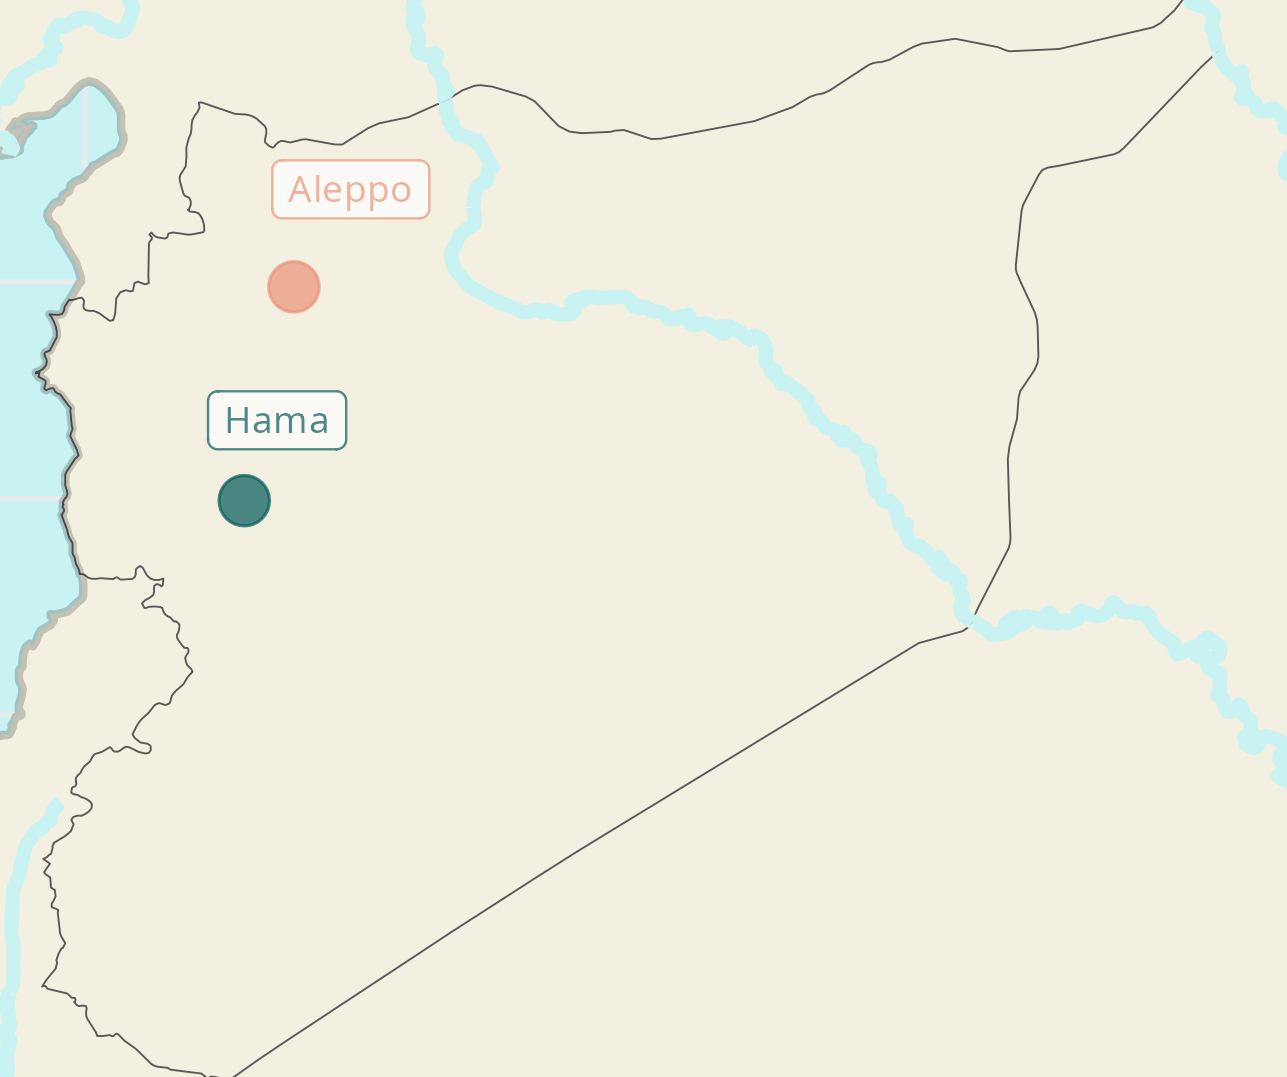
\includegraphics[width=0.8\textwidth]{../../../Mídia/Map02.png}
\end{flushright}

A inscrição HAMA 2 (\autoref{fig:hama2a}) está atualmente locada junto de HAMA
1 e 3 no Eski Şark Eserleri Müzesi, Istabul (no. 7890).

\begin{figure}[h]
	\centering
	\begin{subfigure}{0.49\textwidth}
		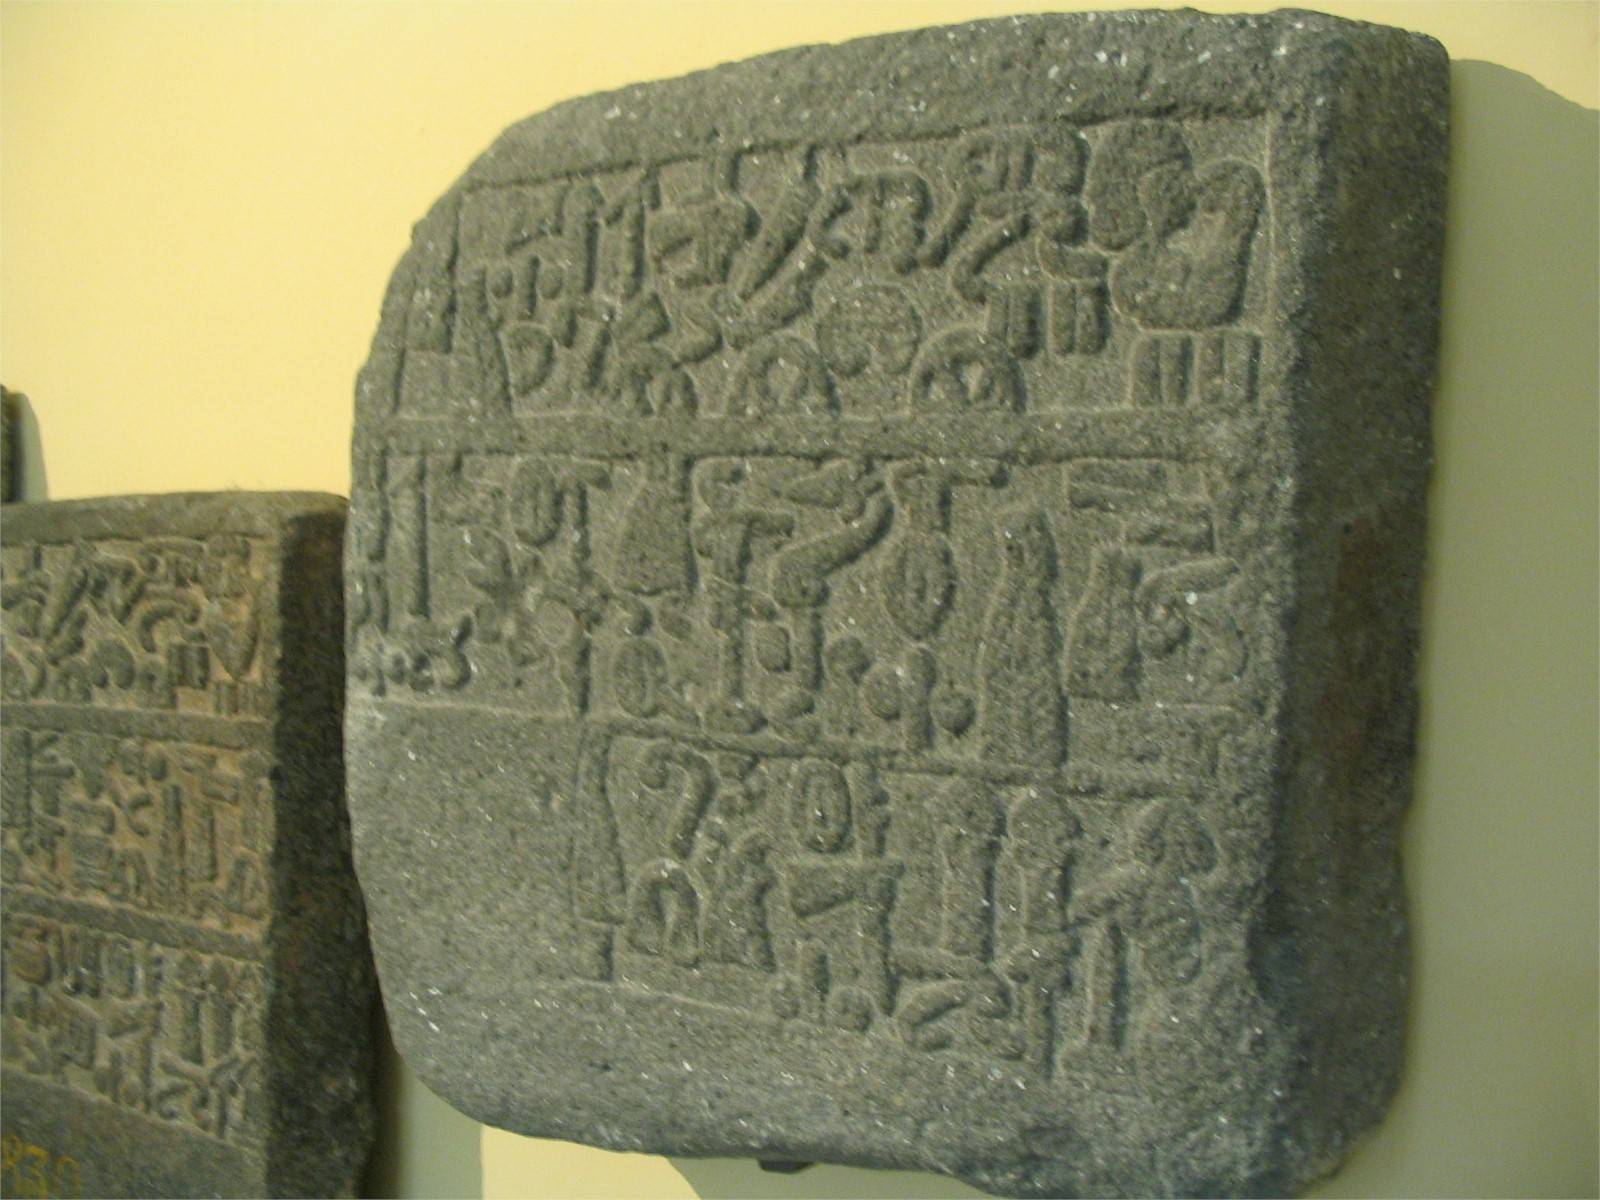
\includegraphics[width=\textwidth]{../../../Mídia/hama08.jpg}
	\end{subfigure}
	\begin{subfigure}{0.49\textwidth}
		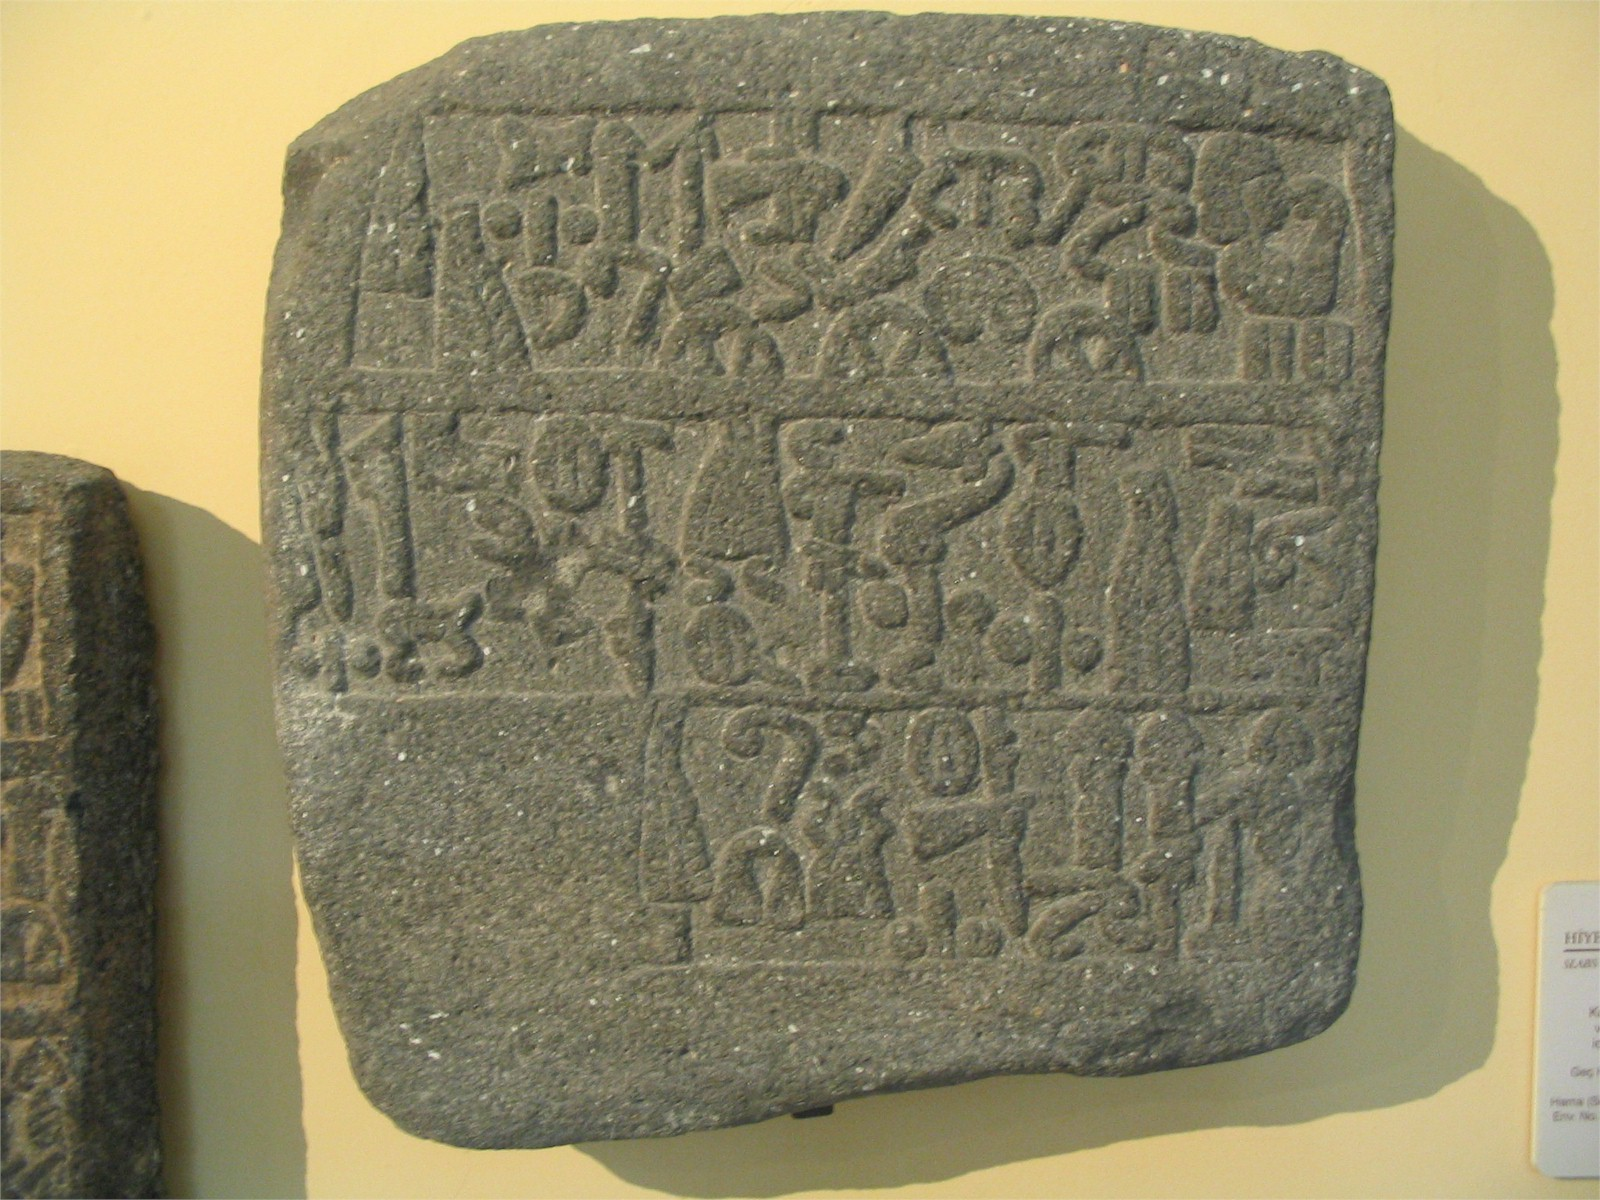
\includegraphics[width=\textwidth]{../../../Mídia/hama09.jpg}
	\end{subfigure}
	\caption[Inscrição HAMA 2]{Inscrição HAMA 2. Dimensões da inscrição:
		0.36\times0.31m.
		Imagens de Bora Bilgin, 2006,
		disponíveis em
		\href{https://www.hittitemonuments.com/hama/}{Hittite Monuments}.
		Edição e traçado em~\citeabbrev*{CHLI11}, pp.\ 411ff.\ e \emph{plates}
		221--2.
	}\label{fig:hama2a}
\end{figure}

\clearpage%


\begin{center}
	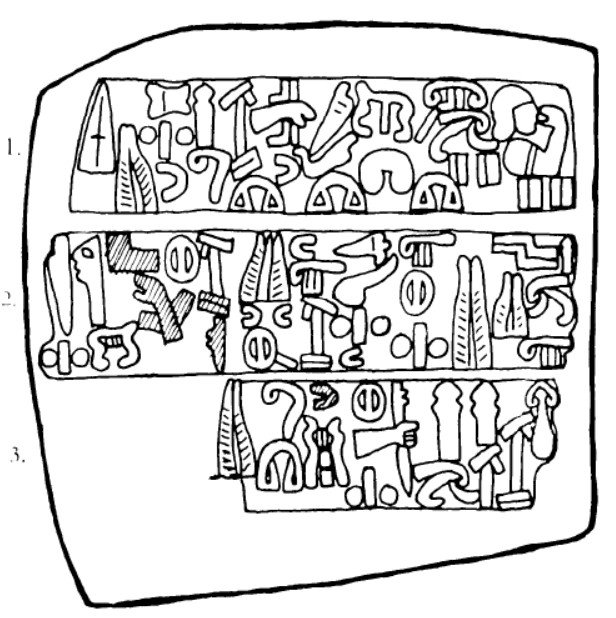
\includegraphics[width=0.85\textwidth]{../../../Mídia/hama14.jpg}
\end{center}

\ex.[]\ag.[1]\LARGE \luwiantrans{EGO-mi} \LARGE \luwiantrans{MAGNUS-ra-da-mi-sa}
\LARGE \luwiantrans{u-ra-hi-li-na-sa} \LARGE \luwiantrans{FILIUS-ni-za-sa}
\LARGE \luwiantrans{i-ma-tu-wa-ni REGIO} \LARGE \luwiantrans{REX}\\
EGO=mi MAGNUS-ra/i-da-mi-sa
u+ra-hi-li-na-sa FILIUS.\emph{NI}-za-sa
{i-ma-tu-wa-ni REGIO} REX\\
amu=mi Uradamis Urhilinas nimuwizas imatuwani hantawatis\vspace{10pt}
\bg.[2]\LARGE \luwiantrans{a=wa} \LARGE \luwiantrans{á-mu}
\LARGE \luwiantrans{AEDIFICARE-mi-ha} \LARGE \luwiantrans{za-a}
\LARGE \luwiantrans{<CASTRUM>-hara-ni-sà-za}
\LARGE \luwiantrans{la-ka-wa-ni-sà-ha-wa REGIO}
\LARGE \luwiantrans{FLUMEN.REGIO-da-i-sà}
\\
a=wa/i á-mu AEDIFICARE+\emph{MI}-ha za-' ``CASTRUM''-hara-ni-sà-za
{la-ka-wa/i-nis=ha=wa/i REGIO} FLUMEN.REGIO-da-i-sà\\
a=wa amu tamaha za harnisa=za | lakawanis=ha=wa hapadis\vspace{10pt}
\bg.[3]\LARGE \luwiantrans{REL-za}
\LARGE \luwiantrans{i-zi-da}
\LARGE \luwiantrans{a-tá-ha-wa}
\LARGE \luwiantrans{ni-ki-ma-sa REGIO}
\\
REL-za i-zi-i-da a-tá-ha-wa/i {ni-ki-ma-sa REGIO}\\
kwa=za izida || anda=ha=wa nikimas

\clearpage%

\ex.[]\ag.[1] amu =mi Uradamis Urhilinas nimuwizas imatuwani hantawatis.\\
\Pro{}1\Sg{} =\Refl{}. U.-\Com{}\Nom{}\Sg{} U.-\Com{}\Gen{}\Sg{} filho-\Com{}\Nom{}\Sg{}
imatuano-\Com{}\Nom{}\Sg{} rei-\Com{}\Nom{}\Sg{}\\
Eu sou Uradamis, filho de Urhilinas, rei imatuano.
\bg.[2] a =wa amu tamaha za harnisa=za,\\
\Conj{} =\Clt{} \Pro{}1\Sg{} construir-1\Sg{}\Pret{} \Pro{}\Neut{}\Acu{}\Sg{}
fortaleza-\Neut{}\Acu{}\Sg{}=\Clt{}\\
E eu (mesmo) construí esta fortaleza,
\bg.[||] lakawanis =ha =wa hapadis\\
L.\Com{}\Nom{}\Sg{} =\Conj{} =\Clt{} fluvial-\Com{}\Nom{}\Sg{}\\
\bg.[3] kwa=za izida,\\
\Rel{}\Neut{}\Acu{}\Sg{}=\Clt{} fazer-3\Sg{}\Pret{}\\
a qual o povo de Laka fez,
\bg.[] anda=ha=wa Nikimas.\\
dento=\Conj{}=\Clt{} N.\Com{}\Nom{}\Sg{}\\
E dentro [dela está] Nikima.

\subsubsection*{Notas}

\paragraph{Linha 1}
\textbf{amu=mi} `eu (sou)': o verbo \emph{as-} `ser, estar' é com frequência deixado
explícito em sentenças nominais e nestes casos costuma-se utilizar a
forma reflexiva do pronome.

\noindent\textbf{imatuwani} `imatuano, proveniente de Hama': em casos muito raros, a
desinência do nominativo singular comum não é expressa na grafia, algo que é
mais comum em inscrições majoritariamente logográficas. A série de inscrições de
Uradamis em Hama (1--3 e 6--7) não utilizam a desinência no gentílico
\emph{imatuwani-}.
Curiosamente, as inscrições de Urhilina, pai de Uradamis, HAMA 4,
RESTAN, QALʿAT EL MUDIQ e HINES,
também não empregam desinência de nominativo no gentílico e, em adição, não
inclui a desinência no nome próprio do rei.
HAMA 8, no entanto, também de Urhilina, emprega a desinência no gentílico, mas
não no nome do rei.
Outras inscrições escavadas em Hama, a saber, MEHARDE e SHEIZAR, empregam
regularmente as desinências.

\noindent\textbf{nimuwizas} `filho': por vezes, assume-se a existência de \emph{niza-}
`filho', um sinônimo de \emph{nimuwiza-} `filho', mas atualmente entende-se que
a grafia <FILIUS-ni-za-sa> e similares represente o logogram FILIUS com o
complemento fonológico \emph{NI} e /za-sa/ representem a fonologia da forma
subjacente, daí que transliteramos FILIUS.\emph{NI}-za-sa
(\citeabbrev*{CHLI3} \emph{ad loc.}).

\noindent\luwiantrans{REX} \textbf{= hantawatis} `rei': a forma sempre é escrita com \luwiantrans{REX} e
nunca é escrita com sua fonologia completa,
apenas com o final \emph{ti-}.\footnote{Raríssimas vezes, com \emph{-ta-}.}
Reconstrói-se a forma subjacente a partir do luvita cuneiforme
\emph{handawati-} `rei'.

\paragraph{Linha 2}
\textbf{amu} `eu': quando o pronome pessoal é utilizado, costuma-se entender que
seja para denotar algum tipo de ênfase, algo como `eu mesmo, fui eu que\ldots{}'.

\noindent\luwiantrans{AEDIFICARE-mi-ha} \textbf{= tamaha} `(eu) construí': note no
traçado da inscrição que \luwiantrans{mi} está \emph{em volta} da mão do
logograma \luwiantrans{AEDIFICARE}. Este uso é frequente para indicar que a
forma subjacente de um certo logograma contém em alguma parte de seu tema um
fonema /m/, independentemente do valor da vogal.\footnote{Por vezes, além
	do complemento fonológico anexado ao logograma, a sílaba /ma/ é representada
	por silabogramas: AEDIFICARE.\emph{MI}-ma-da = \emph{tamada} `ele construiu'
	(KARATEPE 2, §1).}

\noindent\luwiantrans{za-a} \textbf{= za' = za}: o sinal L.450 \luwiantrans{a} funciona
aqui de espaçador.
\textbf{harnisa=za}: \emph{=za} como partícula de dupla marcação do acusativo
neutro singular.

\paragraph{Linhas 2-3}
\textbf{la-ka-wa/i-nis=ha=wa/i REGIO} `povo de Laka': notar que o logograma
determinativo aparece no \emph{final} da escrita fonológica e após a cadeia de
clíticos.

\noindent\luwiantrans{FLUMEN.REGIO-da-i-sà} \textbf{= hapadis} `[terra] fluvial;
alagadiço': nas inscrições HAMA 1--3, parece que os escribas imatuanos,
para deixarem claro que uma sílaba /Ti/ contém uma oclusiva sonora /d/,
escrevem a sequência \luwiantrans{da-i} <da-i> ao invés de empregarem o
silabograma \luwiantrans{ti} <ti>, que poderia representar tanto /ti/ quanto
/di/. No resto do \emph{corpus}, a forma é regularmente escrita com
\luwiantrans{ti} <ti>.\footnote{
	Para uma interpretação contrária, ver~\citet{Simon2019}, que propõe que o
	sinal L.41 possa ter também o vocalismo em /i/, assim <da/i>.
}

\noindent\textbf{lakawanis\ldots{} hapadis} `povo da terra fluvial de Laka': sujeito da
oração relativa iniciada na linha seguinte por \emph{kwa{(n)}=za}.
O motivo da prolepse é incerto, mas pode-se argumentar que a troca de
sujeito\slash{}tópico de Uradamis para o povo de Laka a tenha motivado.

\noindent\textbf{kwa{(n)}=za} `a qual': o referente da relativa é \emph{harnisa=za}
[2].

\noindent\textbf{izida} `fez': o contraste feito entre \emph{amu tamaha} `eu (mesmo)
construí' e \emph{lakawanis hapadis kwa{(n)}=za izida} `o povo da região
fluvial de Laka que a fez' é bastante marcado tanto pela presença do pronome
pessoal quanto pela prolepse do sujeito da oração relativa.
O mesmo ocorre em todas as outras inscrições HAMA 1--3 e 6--7:
\begin{compactitem}
	\item HAMA 1: \emph{hurpadawanis hapadis kwa=za izida} `a qual o povo da região
	fluvial de Hurpada fez'
	\item HAMA 3: \emph{musanipawanis hapadis kwa=za izida} `a qual o povo da região
	fluvial de Musanipa fez'
	\item HAMA 6: \emph{kusunalanzi kwa=za iziyanta} `a qual os kussunalitas fizeram'
	\item HAMA 7: MONS \emph{labarnawanis hapadis kwa=za izida} `a qual o
	povo da região fluvial do monte Labarna fez'
\end{compactitem}

\noindent\textbf{anda=ha=wa} `e dentro [está]': as inscrições HAMA 1, 2 e 7
terminam com esta fórmula seguida de um topônimo.
A fortaleza não poderia cobrir a extensão necessária para conter todos os
territórios nomeados, de modo que se a interpretação for literal `dentro da
fortaleza está X', deve-se entender `dentro está parte da população de X',
talvez aquartelada para defender a fortaleza.
Outra interpretação possível é que em 1, 2 e 7, estejam sendo adicionados outros
povos à lista dos que fizeram, com o sentido `fortaleza a qual o povo Y fez,
\emph{incluindo} o povo de X'.


\begin{flushleft}
	\noindent \textbf{Transcrição}\\
	\noindent [1] \emph{amu=mi Uradamis Urhilinas nimuwizas imatuwani hantawatis.}\\
	\noindent [2] \emph{a=wa amu \mbox{tamaha} za harnisa=za,}\\
	\noindent [3] \emph{lakawanis=ha=wa hapadis kwa=za izida,}\\
	\noindent [4] \emph{anda=ha=wa \mbox{nikimas}.}


	\noindent \textbf{Tradução}\\
	\noindent [1] ``Eu sou Uradamis, filho de Urhilina, rei imatuano.\\
	\noindent [2] Eu mesmo construí esta fortaleza,\\
	\noindent [3] (e) a qual o povo de Laka fez\\
	\noindent [4] e dentro dela está Nikima.''
\end{flushleft}


\noindent\textbf{Vocabulário}
\begin{multicols}{2}
	\noindent \emph{amu-} (\emph{pron.1sg.}) eu\\
	\noindent \emph{anda} (adv.) dentro\\
	\noindent \emph{Uradami}- (NP com.) Uradamis\\
	\noindent \emph{Urhilina}- (NP com.) Urhilina\\
	\noindent \emph{hantawati}- (subst.com.) rei\\
	\noindent \emph{hapadi}- (adj.) fluvial\\
	\noindent \emph{harnisa}- (subst.neut.) fortaleza\\
	\noindent \emph{imatuwani}- (adj.) proveniente de Hama\\
	\noindent \emph{izi{(ya)}}- (v.t.) fazer, criar\\
	\noindent \emph{lakawani}- (adj.) proveniente de Laka\\
	\noindent \emph{nikima-}- (subst.com., topônimo) Nikima\\
	\noindent \emph{nimuwiza}- (subst.com.) filho\\
	\noindent \emph{tama}- (v.t.) construir
\end{multicols}
